%=======================+=========================
%================  Reconstruction  ================
%=================================================


\section[Event reconstruction]{Event reconstruction \label{sec:reconstruction}}

% Copy from GlueX-doc-3108
% "Production and Analysis of GlueX Data"
% TODO: UPDATE for 2017

During and after the experimental running, \GX~uses the computer center batch farm at Jefferson Lab to perform data monitoring, event reconstruction, and physics analyses.  For data monitoring, we study the detector hit occupancies, calibration and reconstruction quality, and experimental yields and resolutions for several physics channels.  We monitor a subset of the data as soon as it is saved to tape via batch farm jobs submitted by cron jobs.  Every few weeks, we launch monitoring processes on a subset of the data to study improvements from ongoing calibrations and reconstruction software improvements.  The histograms produced by these monitoring jobs are displayed on a web site and ROOT files are available for download, enabling the collaborators to easily study the quality of the data. 

Every few months we perform a major reconstruction launch over all of the data, linking the hits in the various detector systems to reconstruct particles in the physics events.  Monitoring plots from these launches are also published to the web. Finally, we regularly perform analysis launches over the reconstructed data, where a JANA plugin is used to filter out reactions that were previously specified by users in a web form. The results of these launches are saved in reaction-specific ROOT TTrees for further analysis.

For all launches, JANA is run multithreaded to make efficient use of the available computing resources. Figure~\ref{fig:offline_monitorA} shows the multithreaded scaling from our monitoring launches. It is near the theoretical limit for jobs that use a number of threads that is less or equal the number of physical cores on the processor. By using hyperthreads, a smaller but still significant gain is achieved.
%SWIF is used to manage the batch farm jobs, and is queried to study the performance of the launches.  Figure~\ref{fig:farm-time} shows how many batch farm jobs were in each processing state as function of time our latest reconstruction launch.
All file outputs are written to a write-through cache system, which is ultimately backed up to tape.

\begin{figure}[h!]\centering
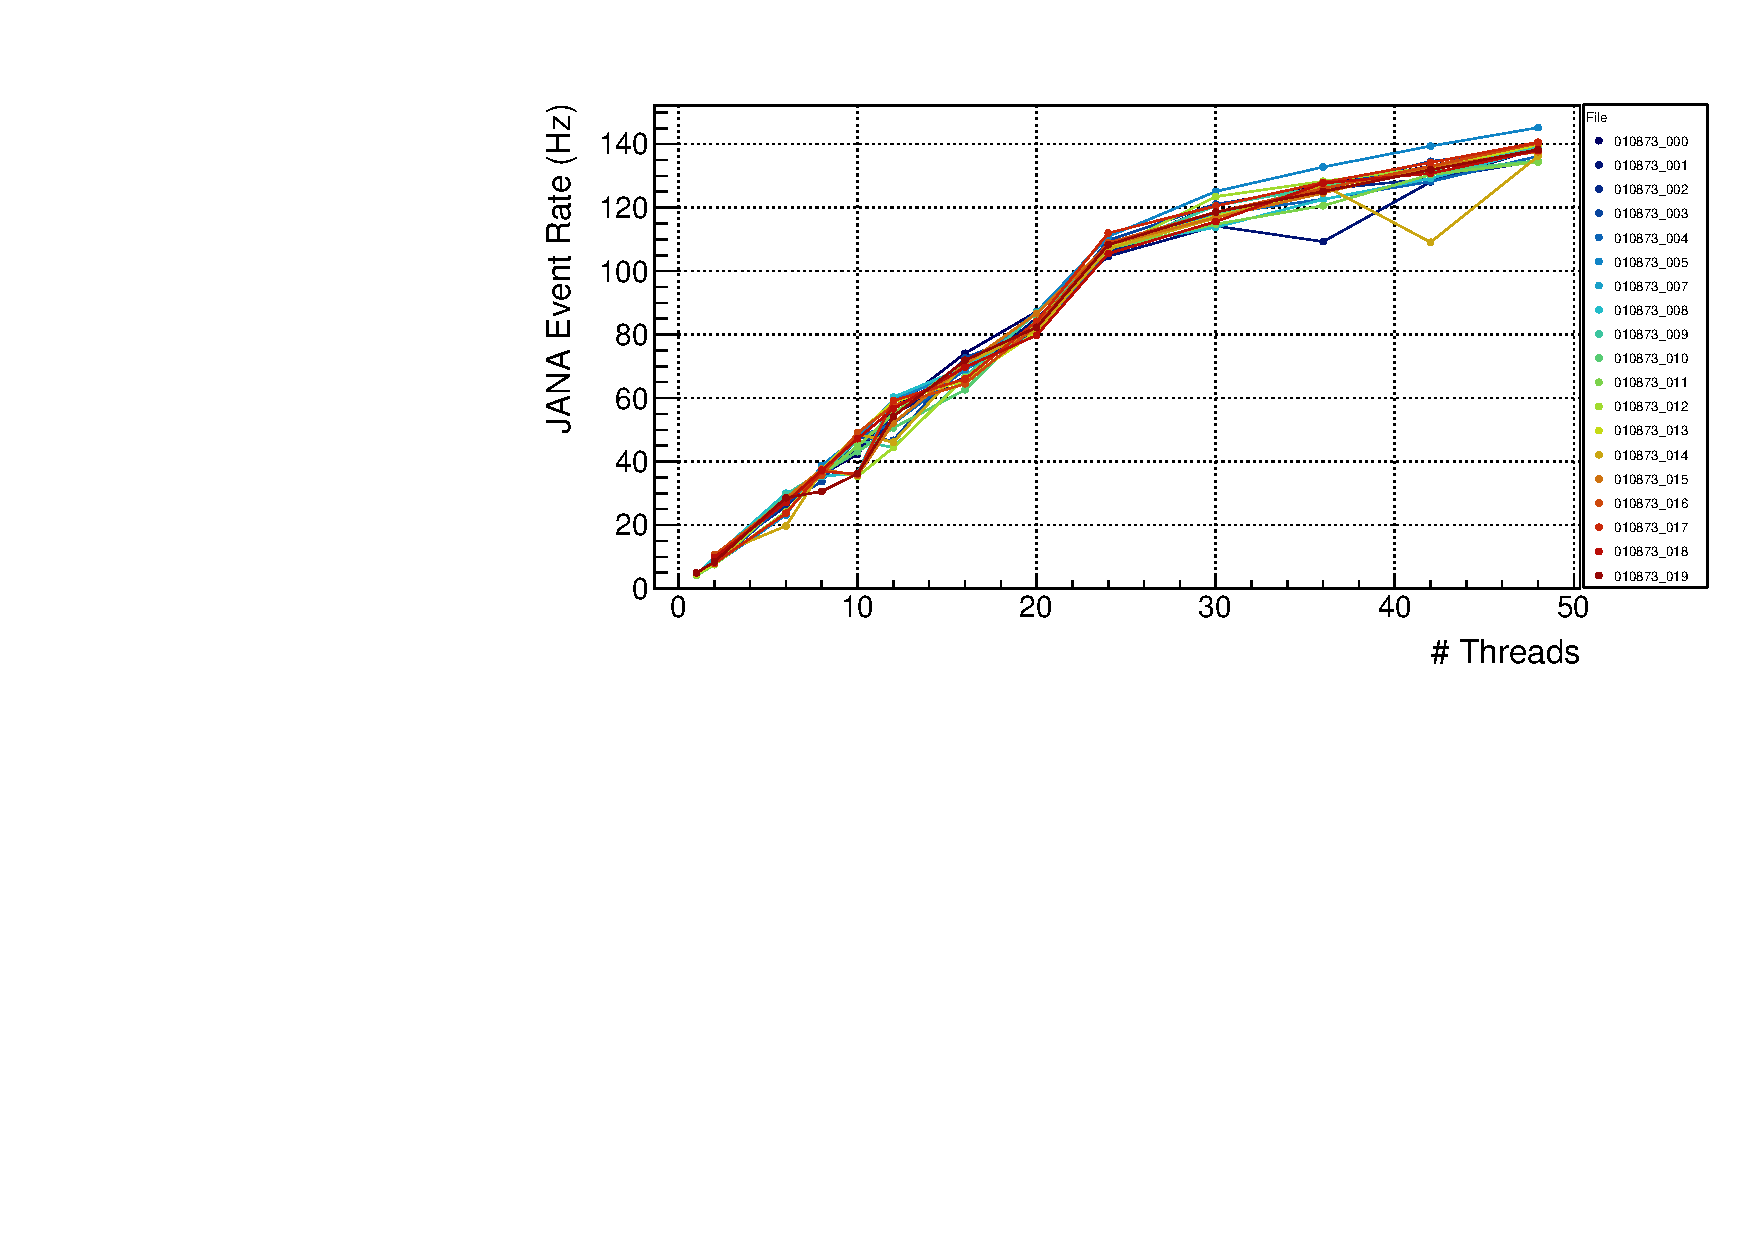
\includegraphics[width=0.7\textwidth]{figures/OfflineMonitor_PlotA.pdf}
\caption[]{\label{fig:offline_monitorA}The scaling of program performance as a function of the number of processing threads. The computer used for the test consisted of 24 full cores (Intel x86\_64) plus 24 hyper threads}
\end{figure}

The series of steps in the production of \GX~data will be described in the following. In its initial phase, \GX~recorded about 1400 separate physics-quality runs having a total data footprint of about 3 petabytes. The data acquisition system saved the data in $19$ gigabyte files, with all runs consisting of multiple files (typically $100$ or more). Figure~\ref{fig:production_overview} shows an overview of the different production steps for \GX~data. 

\begin{figure}[h!]\centering
%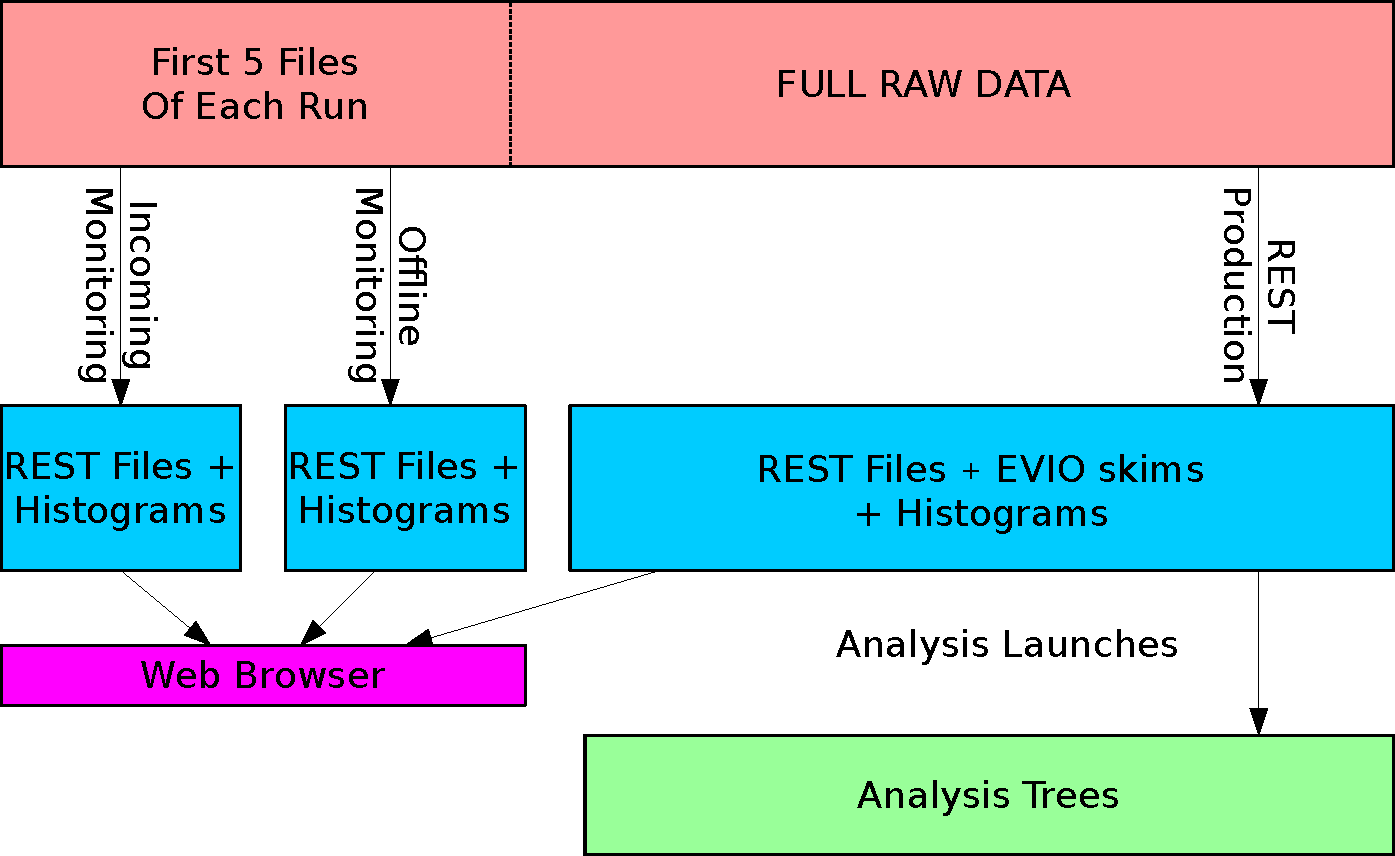
\includegraphics[width=0.8\textwidth]{figures/Production_generic.pdf}
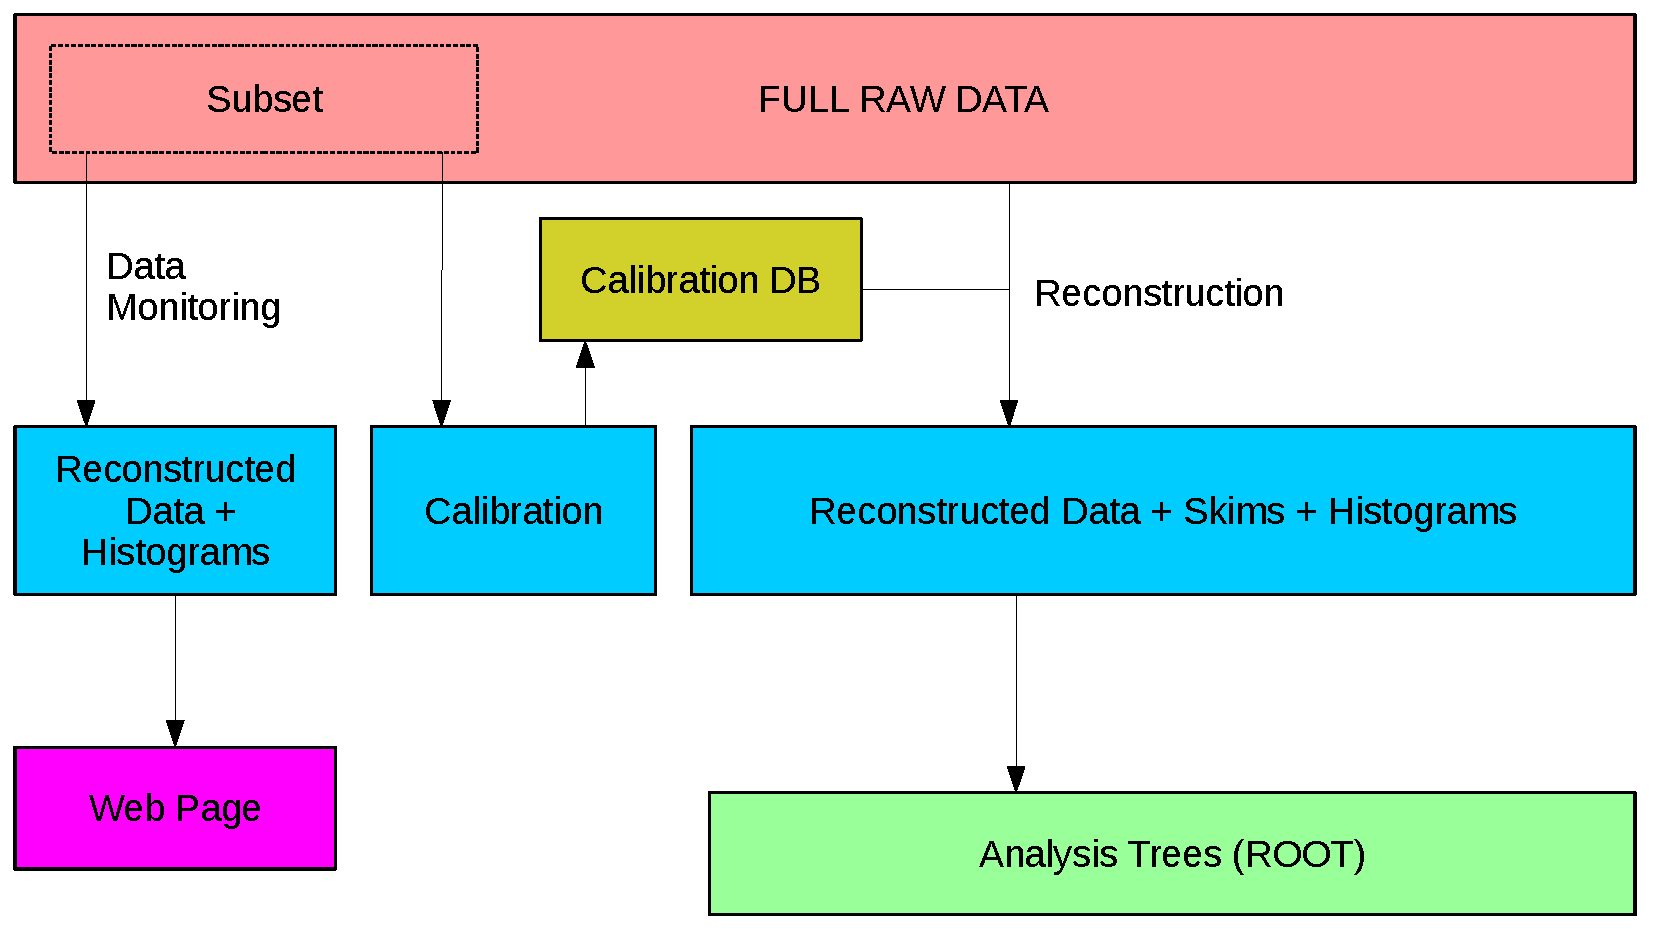
\includegraphics[width=0.9\textwidth]{figures/production_overview_calib_v2.pdf}
\caption[]{\label{fig:production_overview}Production flow chart for \GX~data.} 
\end{figure}

\subsection{Calibration pass \label{sec:reccalibration}}

Two types of calibration jobs are run, depending on the complexity of the calibration procedures.  Simple, well-understood calibrations such as timing alignment between individual channels and subdetectors or drift chamber gain and time-to-distance calibrations, can be performed with one file of data per run.  These procedures are run either in the online environment or on the batch farm, and can be run several times as needed due to improvements in reconstruction algorithms or other calibrations.

More complicated calibration procedures, such as calorimeter gain calibration, require more data and are often iterative procedures, requiring several passes through the data.  The raw data is processed as it arrives on the batch farm resulting in histograms or in selected event data files in EVIO or ROOT tree format.  Many of these outputs require that charged particle tracks be reconstructed, but because of the computationally intensive nature of track reconstruction at \GX, the available computing resources at JLab are insufficient for fully reconstructing all of the raw data as it comes in.  Therefore, only about $10-20$\% of the data has the full suite of calibration procedures applied.  The rest has a limited set of procedures, mostly focused on separating out events collected by specialized triggers. 
The individuals responsible for specific detector calibrations are then responsible for analyzing the skimmed data.

\subsection{Monitoring pass \label{sec:recmonitoring}}

The red-colored box at the top of Fig.~\ref{fig:production_overview} represents the experimental data that has been copied to the computer center. The left-hand section of the box labeled ``subset" represents the first five files of each run, which are run through the offline monitoring processes. These monitoring jobs are first run during the run to check the quality of the data, but are also run after major changes to calibrations or software to validate those changes. These jobs produce both Reconstructed Events Storage (REST) files and root histogram files for checking the detector and reconstruction performance.

\subsection{Reconstruction pass \label{sec:recreconstruction}}

When the data is sufficiently well calibrated, we carry out a full production pass on the physics quality data. In the total \GX~data set, about 1400 of the runs were deemed physics quality. The remaining were short runs which were related to engineering and commissioning tests of the experiment. We note that while this number is small compared to the total number of runs, it includes the vast majority of all data recorded during the running period, representing about 3 petabytes. All of these files were reconstructed using several computing resources with an equivalent to more than 20 million core-hours combined. They produced more than $500$ terabytes of REST data files. The large reduction is size, about a factor of six, from collected event data to physics data files allows us to  more quickly and efficiently carry out physics analyses on the data.
%, and is also small enough to be fully exported to off-site computer centers, see section~\ref{sec:remote-dist} (not really).

In the REST production, we included a series of detector performance studies that required access to raw data and that would not be possible on the reconstructed data alone. Many improvements to software and detector calibration resulted from these studies. Similar studies can be made with simulated data to match and assess the detector acceptance.

\subsection{Offsite Reconstruction}
\label{sec:recoffsite}

Production processing of \GX~data utilizes offsite HPC resources in addition to the onsite farm at JLab. Specifically, the National Energy Research Super-computing Center (NERSC) and the Pittsburgh Super-computing Center (PSC). For NERSC, the total allocation used for AY2019 was 53M NERSC units which was used to process 70.5k jobs. This is equivalent to approximately 9M core-hours on a Intel x86\_64 processor. The jobs were run on NERSC's Cori II system which is comprised of KNL (Knight's Landing) processors. The PSC allocation was awarded through the XSEDE allocation system in the last quarter of CY2019 for 5.9M SU's. Only 0.85M SU's were used in 2019 to run 7k jobs on the PSC Bridges system or about 10\% of what was processed at NERSC. Figure \ref{fig:production_offsite_rate_vs_nthreads_NERSC} shows how the event processing rates scaled well with the number of processing threads for both NERSC and PSC. Jobs run at both of those sites were assigned entire nodes so the number of processing threads used was equal to the total number of hardware threads.

\begin{figure}[h!]\centering
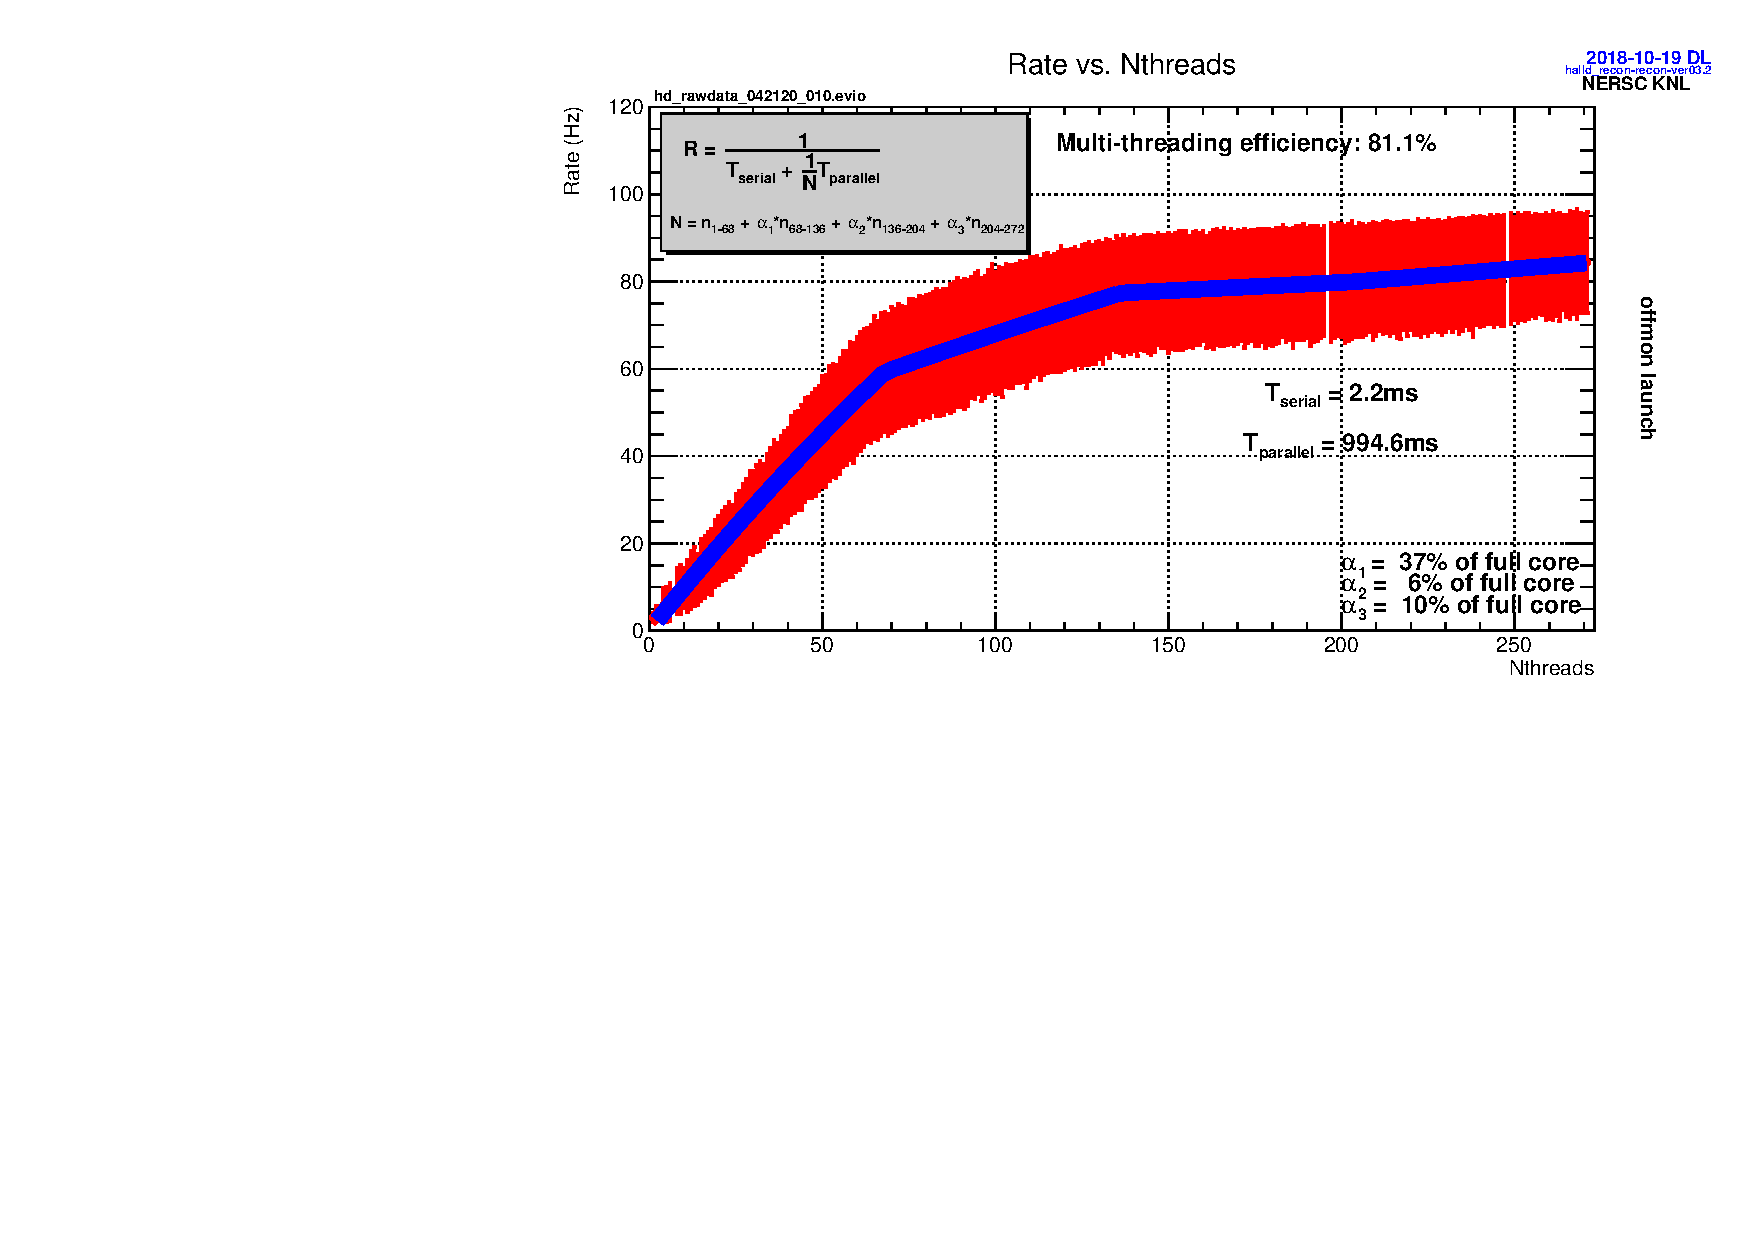
\includegraphics[width=0.49\textwidth]{figures/production_offsite_rate_vs_nthreads_NERSC.pdf}
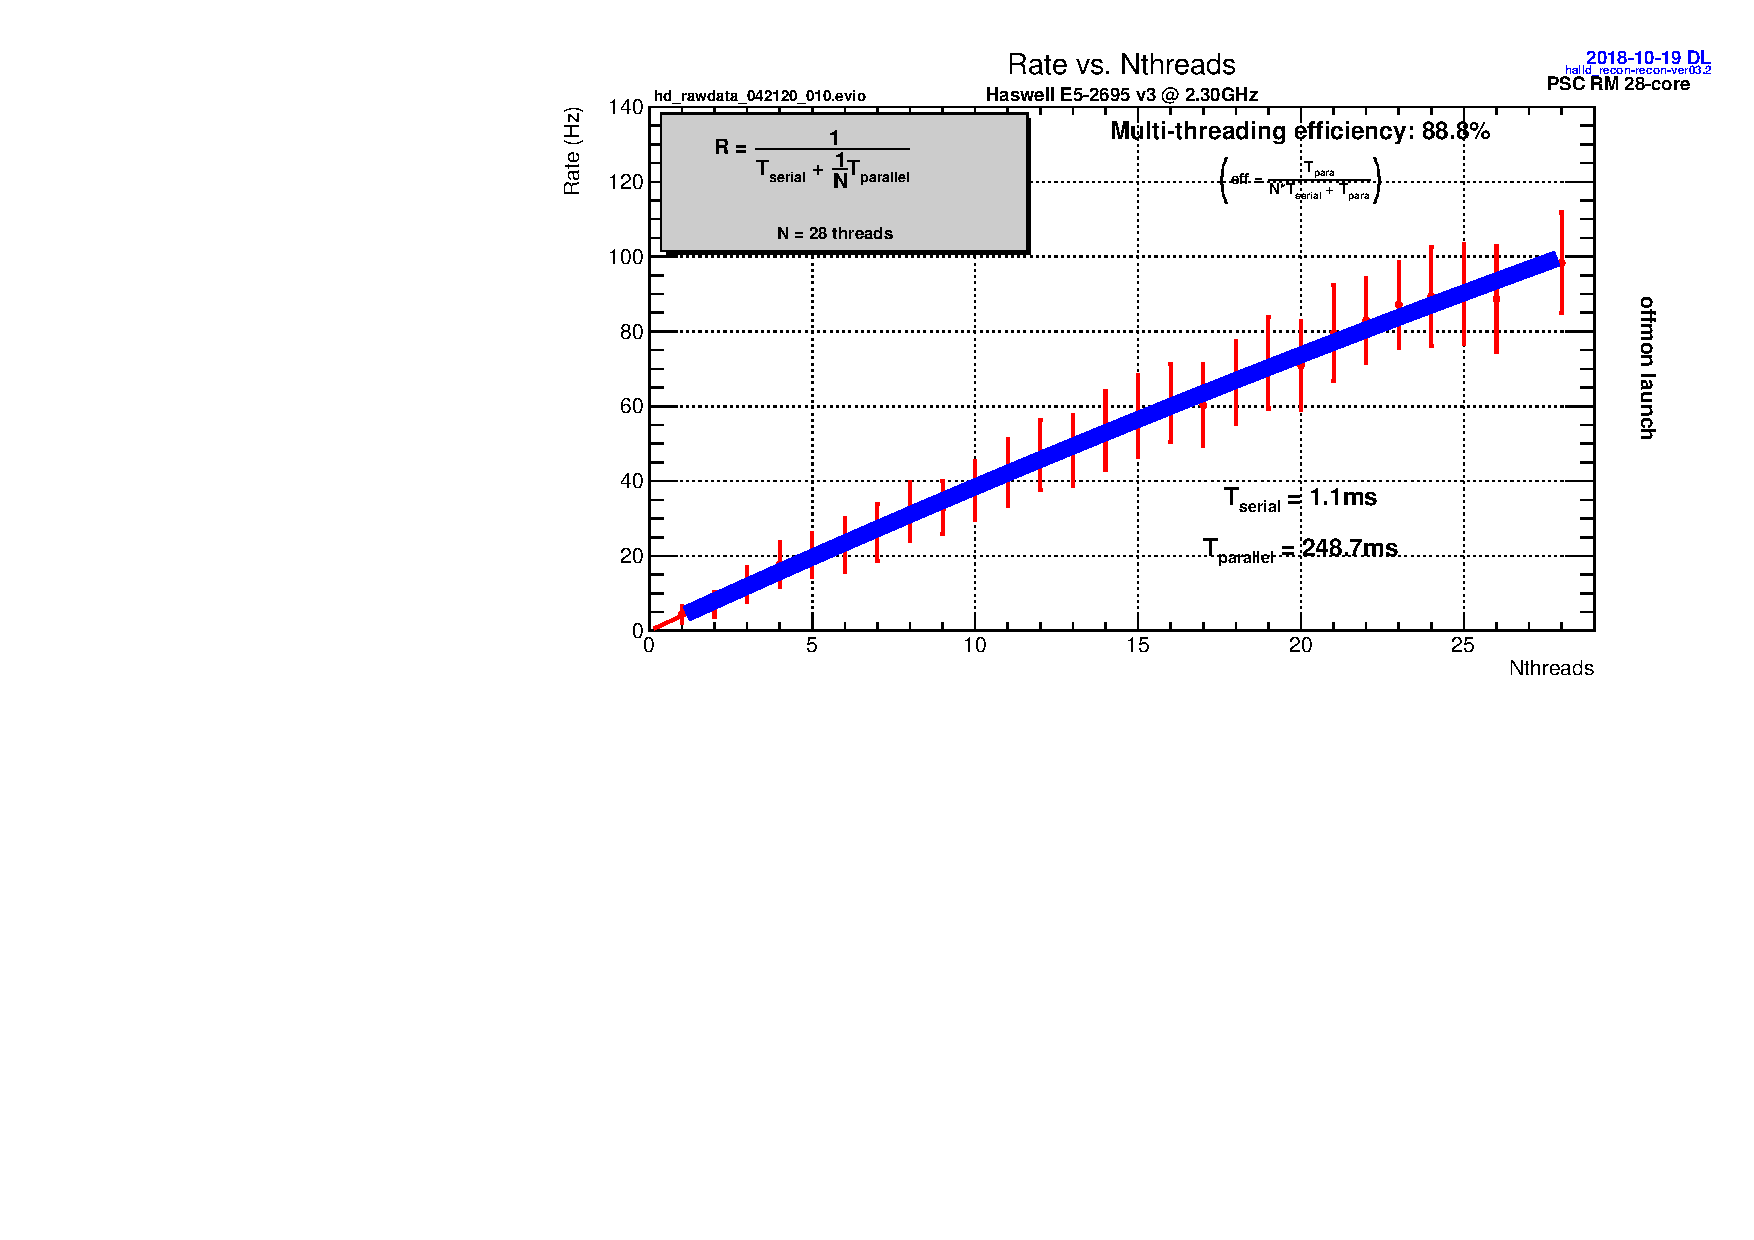
\includegraphics[width=0.49\textwidth]{figures/production_offsite_rate_vs_nthreads_PSC.pdf}
\caption[]{\label{fig:production_offsite_rate_vs_nthreads_NERSC}Event processing rate vs. number of threads for reconstruction jobs on NERSC Cori II (left) and PSC Bridges (right). The structure in the NERSC plot is due to the KNL architecture having 4 hardware threads per core. For PSC Bridges, hyper-threading is disabled so no structure is observed.} 
\end{figure}

Container and distributed file system technologies were used for offsite processing. The software binaries as well as calibration constants, field maps etc. were distributed using the CERN-VM-file system (CVMFS). The binaries were all built at JLab using a CentOS7 system. A very lightweight Docker container was made based on CentOS7 that had only a minimal number of system RPMs installed. All other software, including 3rd party packages such as ROOT, were distributed via CVMFS. This meant changes to the container itself were very rare (about once per year). The Docker container was pulled into NERSC\'s Shifter system without modification. The same container was used to create a Singularity container used at both PSC and on the OSG for \GX~simulation jobs.

Raw data was transferred from JLab to the remote sites using Globus,  which uses GridFTP. The Globus tasks were submitted and managed by the SWIF2 workflow tool written by the JLab Scientific Computing group. SWIF2 was needed to manage the data retrieval from tape, transfer to the remote site, submission of remote jobs, and transfer of processed data back to JLab. Disk space limitations at both JLab and the remote sites meant only a portion of the data set could be on disk simultaneously. Thus, SWIF2 had to manage the jobs through all stages of data transfer and job submission.

% too much detail?
% Figure \ref{fig:production_offsite_RunPeriod2018-08_batch01_iNjobs_vs_time} shows the integrated number of jobs processed over several days of a campaign. Campaigns were broken up into batches of jobs which could then be assigned to different facilities for processing. The number of jobs processed per day varied, particularly at NERSC where the footprint of jobs from other fields competing for the resource changed daily.

%\begin{figure}[h!]\centering
%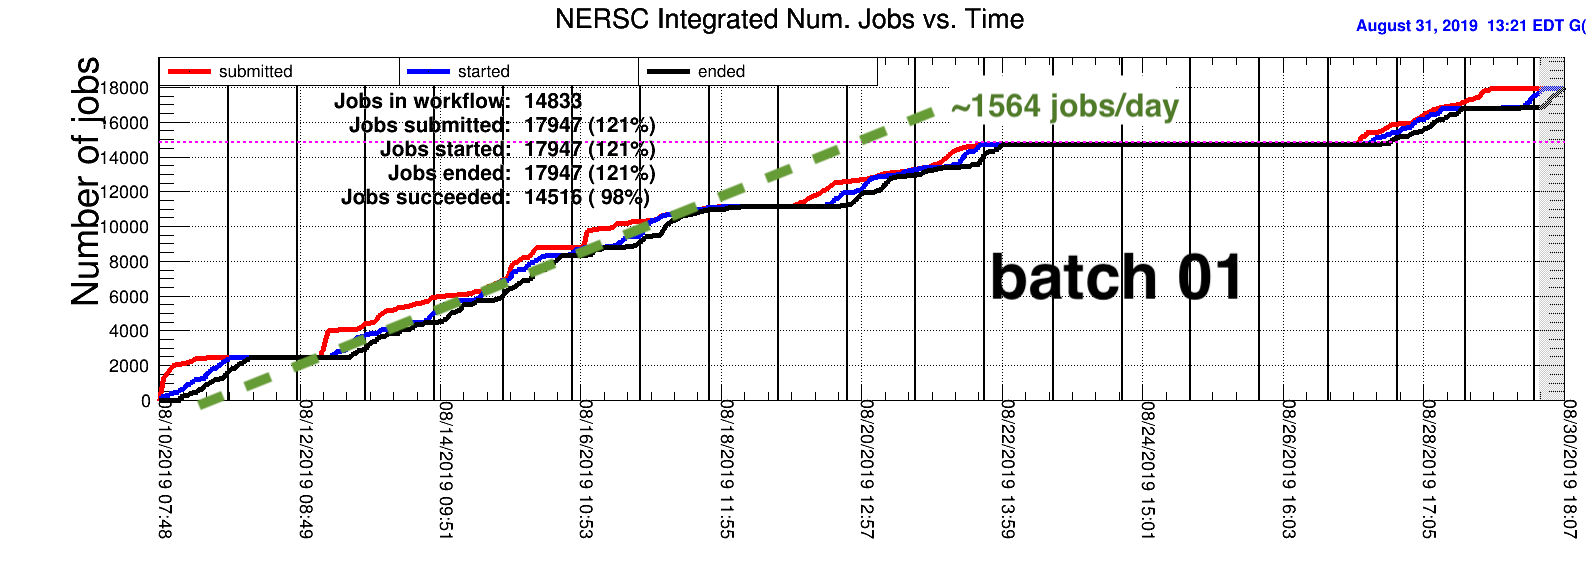
\includegraphics[width=0.75\textwidth]{figures/production_offsite_RunPeriod2018-08_batch01_iNjobs_vs_time.png}
%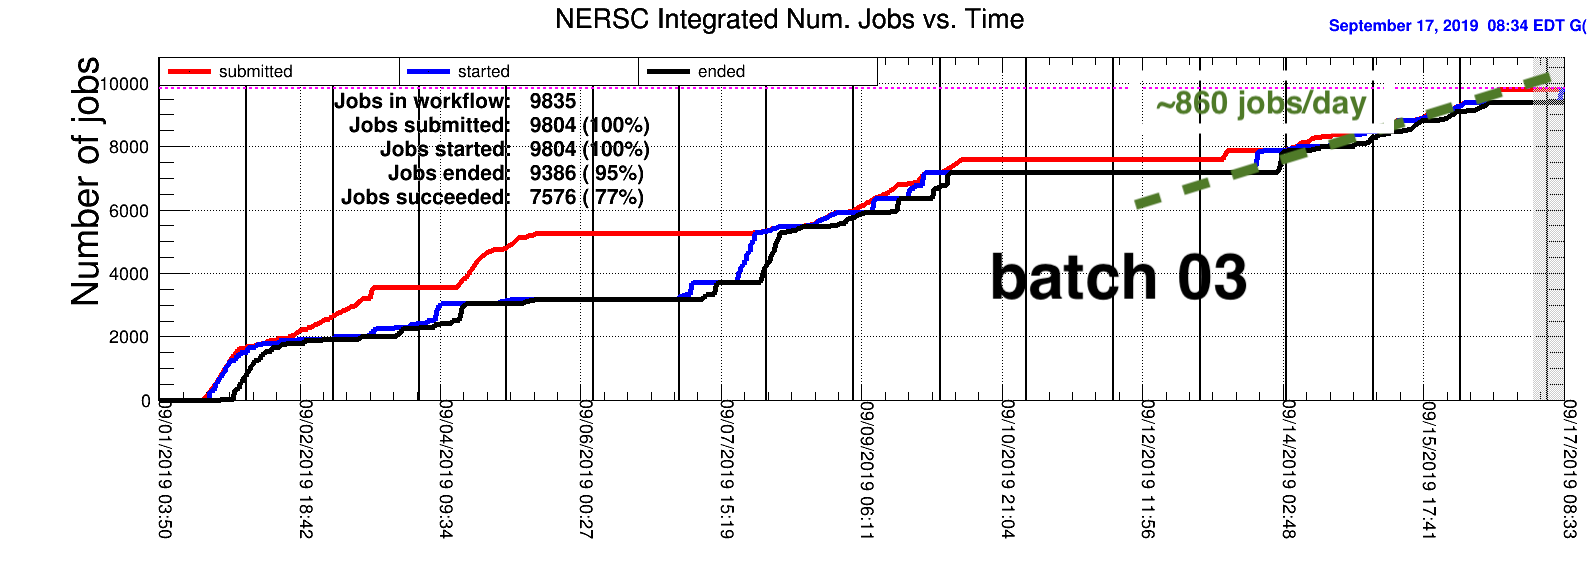
\includegraphics[width=0.75\textwidth]{figures/production_offsite_RunPeriod2018-08_batch03_iNjobs_vs_time.png}
%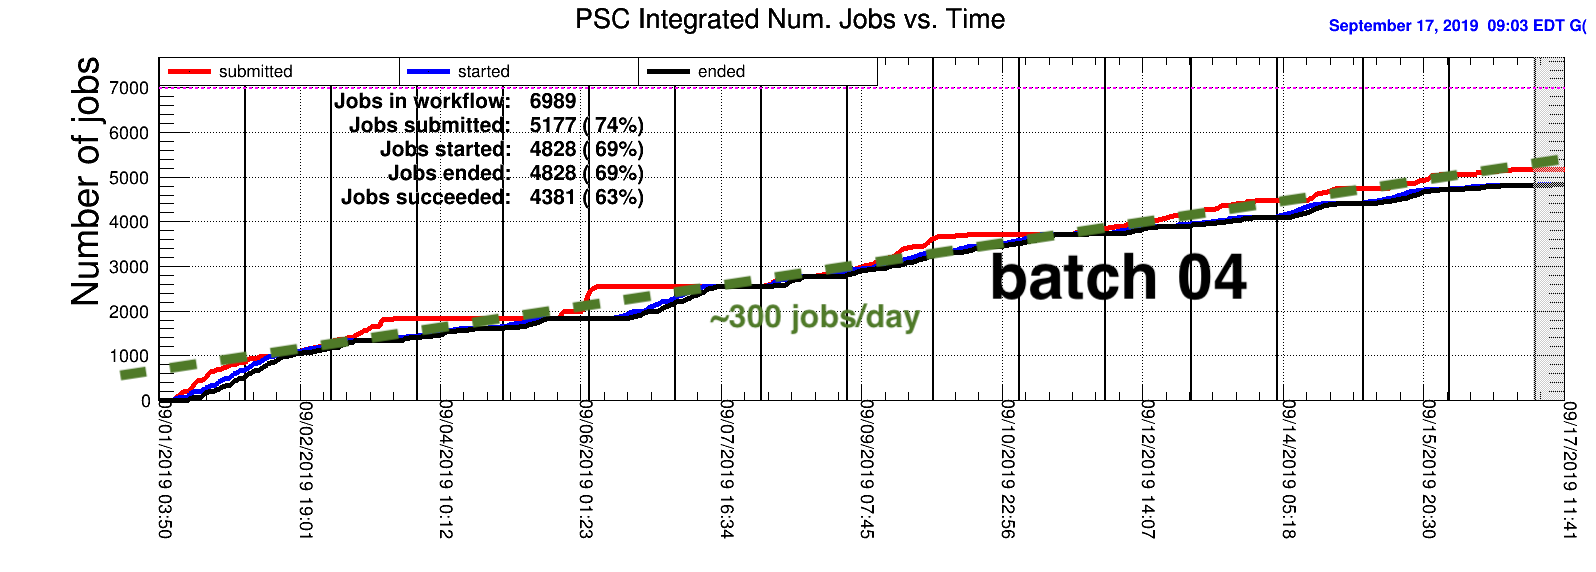
\includegraphics[width=0.75\textwidth]{figures/production_offsite_RunPeriod2018-08_batch04_iNjobs_vs_time.png}
%\caption[]{\label{fig:production_offsite_RunPeriod2018-08_batch01_iNjobs_vs_time}Integrated jobs processed for batches of jobs run at offsite HPC facilities. Top: Jobs run at NERSC Cori II using the ``regular'' queue. Middle: Jobs run at NERSC Cori II using the ``low'' priorty queue. Bottom: Jobs run at PSC Bridges.} 
%\end{figure}


\subsection{Analysis pass \label{sec:recanalysis}}

The full reconstructed (REST) data is too large to be easily handled by individual analyzers. For that reason, we developed a system to analyze data at Jefferson Lab and extract final-state specific ROOT trees. This step is represented by the right-hand green box at the bottom of Figure~\ref{fig:production_overview}.

Users can specify individual reactions via a web interface (see Fig.~\ref{fig:production_analysis}). Periodically, the submitted reactions are downloaded into a configuration file, which steers the analysis launch. For each reaction, the \GX~analysis library inside the JANA framework creates possible particle combinations from the reconstructed charged tracks and showers saved in the REST format. Common selection criteria are applied for exclusivity and particle identification before performing a kinematic fit, using vertex and four-momentum constraints. Displaced vertices and inclusive reactions are also supported. Objects representing successful particle combinations (e.g. $\pi_0 \rightarrow \gamma\gamma$) and other objects are managed in memory pools and can be reused in between different channels to reduce the overall memory footprint of the process. With this scheme, we are able to bundle up to one hundred different reactions into one launch over the reconstructed data.

If the kinematic fit converged for one combination of tracks and showers, the event is stored into a reaction-specific but generic ROOT tree, made accessible to the whole collaboration. The total size of these ROOT trees for the full data set strongly depend on the selected reaction, but they are small enough to be copied to the user's home institution for a more detailed analysis.

\begin{figure}[h!]\centering
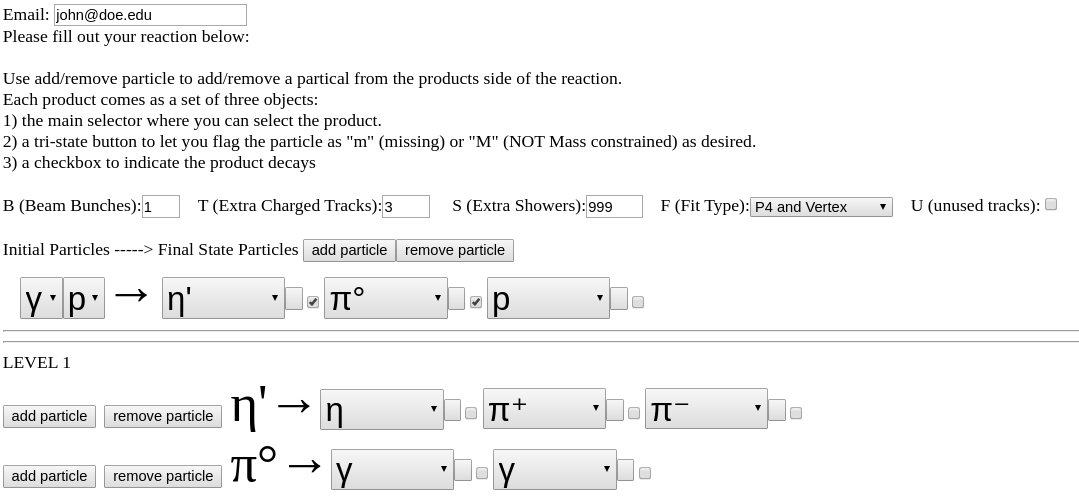
\includegraphics[width=\textwidth]{figures/analysis_submit_form.png}
\caption[]{\label{fig:production_analysis}Analysis submission browser form.} 
\end{figure}